%!TEX root = report.tex
Running the Min-Over algorithm on a student perceptron yields a few interesting results. We present several results we have found here and discuss them in section~\ref{sec:discussion}. 

In all cases the number of neurons was 20, the values of $\alpha = (0.1, 0.2, 0.3, \ldots 4.9, 5.0)$. The value of delta was $10^{-5}$ and the value of $\text{n}_{\text{max}} = 200$.

\myfigure{
	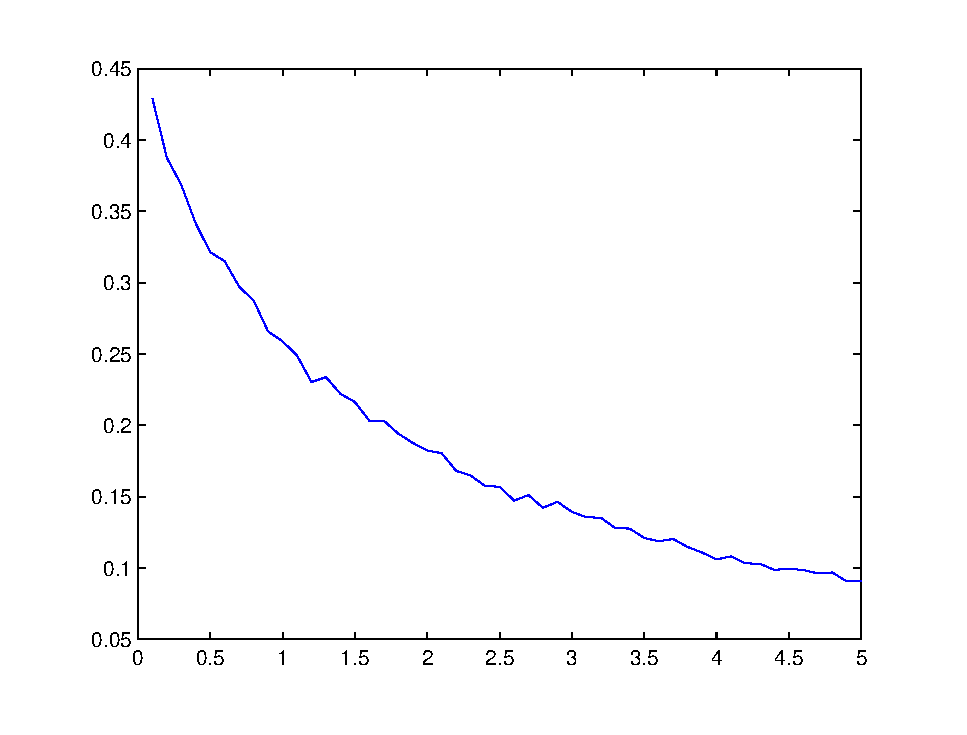
\includegraphics[width=\columnwidth]{learningcurve_100_innerloops.eps}%
	\figcaption{The learning curve of the student perceptron. It shows the generalization error against $\alpha$. This is the average of 100 trainings per $\alpha$-value}
	\label{fig:learningcurve}
}

Figure~\ref{fig:learningcurve} shows the learning curve of the perceptron. It shows the generalization error against the value of $\alpha$, thus the number patterns over the number of input neurons. 

The generalization error determines the probability that disagreement occurs between the teacher perceptron and the student perceptron. Figure~\ref{fig:generalizationerror} plots the generalization error as a function of the time.
\myfigure{
	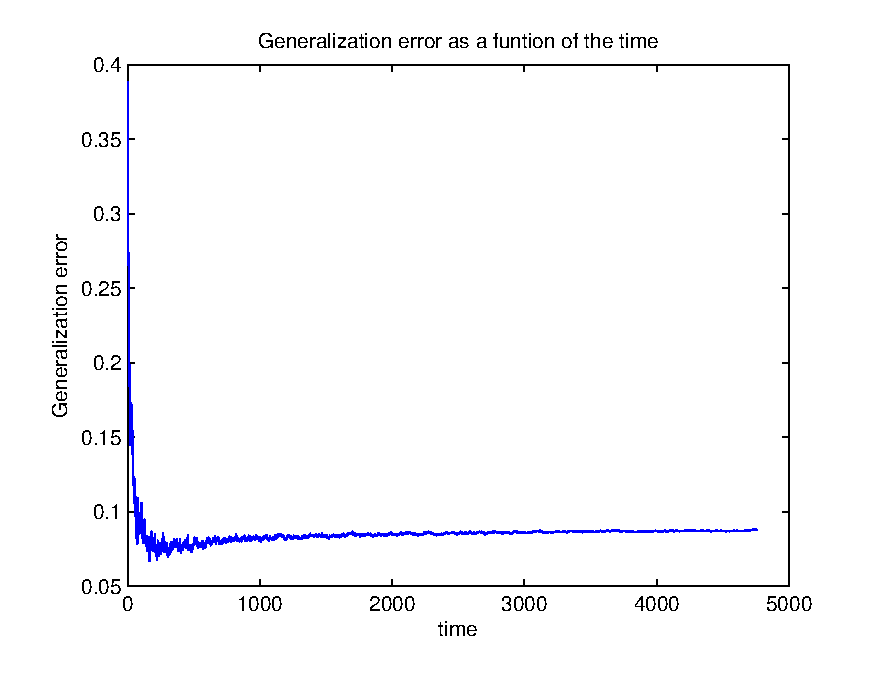
\includegraphics[width=\columnwidth]{generalizationerror.eps}%
	\figcaption{The generalization error as a function of the time. Note it converges quite fast.}
	\label{fig:generalizationerror}
}

It can be seen in figure~\ref{fig:generalizationerror} that error converges relatively fast towards a certain value. We have found that for noise-free learning the value it converges towards is around  $\frac{1}{10}$.

Moreover, the Min-Over algorithm has also been run on noisy data. There was 5\% noise added to the data. This means that approximately 5\% of the labels $S^{\mu}_R$ had a flipped sign as opposed to what the teacher perceptron trained. This should prove the robustness of the algorithm.
\myfigure{
	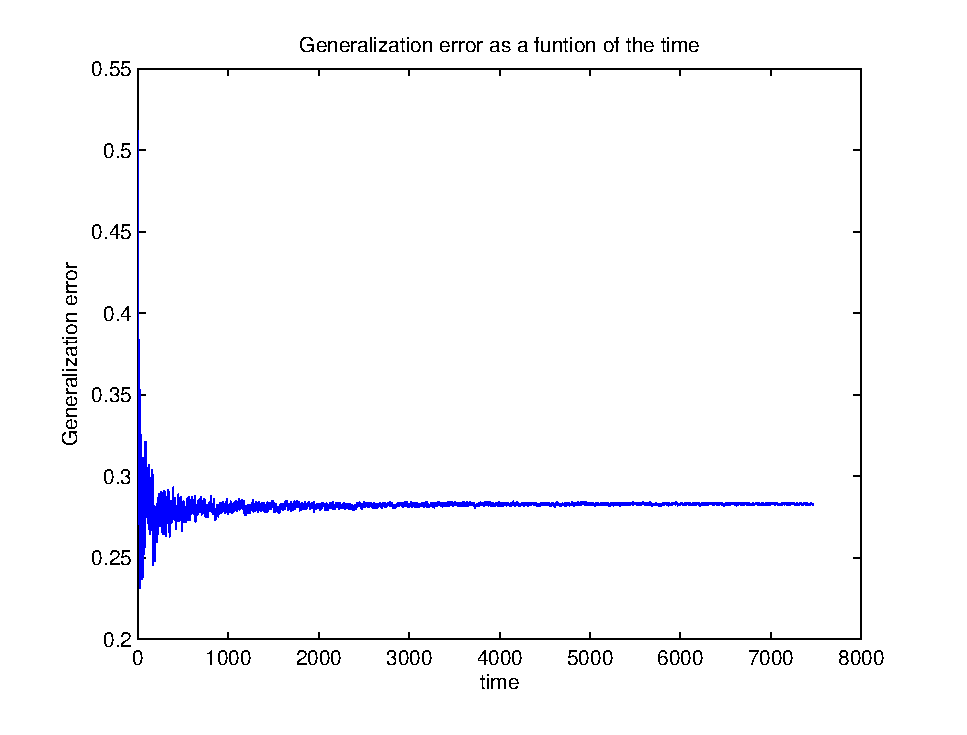
\includegraphics[width=\columnwidth]{generalizationerror_noisy.eps}%
	\figcaption{The generalization error as a function of the time, with 5\% noise added}
	\label{fig:generalizationerror_noisy}
}
Figure~\ref{fig:generalizationerror_noisy} shows the generalization error of the perceptron training with noisy data. In comparison with figure~\ref{fig:generalizationerror} it is visible that the system still converges to some value, but the convergence value is higher than with non-noisy training data. 

\myfigure{
	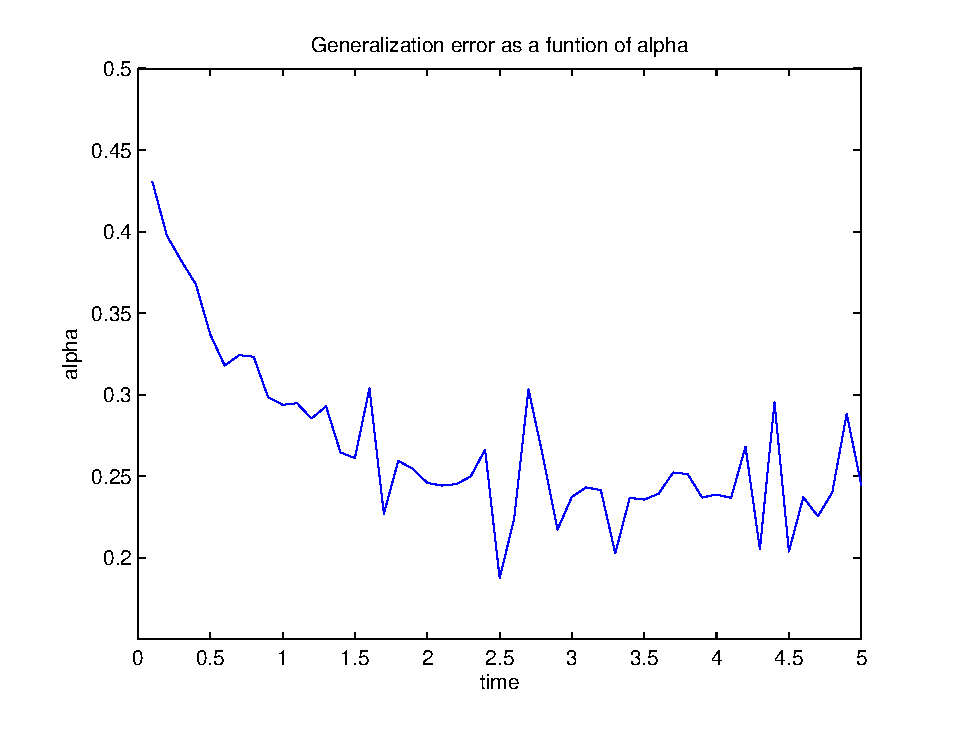
\includegraphics[width=\columnwidth]{learningcurve_noise.eps}%
	\figcaption{Learning curve of a student perceptron where 5\% noise is added to the data}
	\label{fig:noisecurve}
}
Figure~\ref{fig:noisecurve} shows the learning curve as figure~\ref{fig:learningcurve} does, but 5\% noise is added. They are somewhat similar but the curve of figure~\ref{fig:noisecurve} is less smooth as well as having an overall higher generalized error value.